\section{Introduction}

\begin{frame}{Why static binary analysis?}
  \tikzset{every node/.style=draw,->}
  \begin{columns}
  \column{.3\textwidth}
  \begin{block}{Static}
    \centering
    \pause
    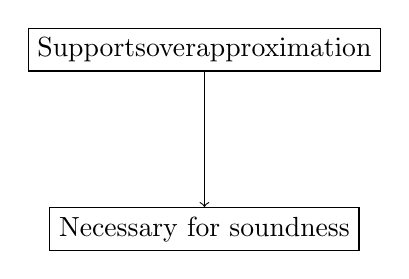
\begin{tikzpicture}
      \node (a) {\makecell{Supports\\\alert{overapproximation}}};
      \pause
      \node [below=2cm] (b) {\makecell{Necessary for \alert{soundness}}};
      \draw (a) -- (b);
    \end{tikzpicture}
  \end{block}

  \column{.58\textwidth}
    \begin{block}<4->{Binary} % Using + wasn't working right; this setup doesn't preserve positioning the way I want but it least puts everything on the right slides
      \centering
      \begin{tikzpicture}
        \node<5-> (a) {Analysis w/o source};

        \node<6-> [below left=.5cm of a] (b1) {Legacy progs};
        \draw<6-> (a) -- (b1);

        \node<7-> [below=.5cm of a] (b2) {Reverse eng.};
        \draw<7-> (a) -- (b2);

        \node<8-> [below right=.5cm of a] (b3) {\makecell{No compiler\\in \glsxtrshort{tcb}}};
        \draw<8-> (a) -- (b3);
      \end{tikzpicture}
    \end{block}
  \end{columns}
\end{frame}

\begin{frame}{Why \glsxtrlong{cfr}?}
  \centering
  \begin{tikzpicture}[every node/.style={draw,ellipse},->]
    \node (prelim) {No indirection in prelim};
    \pause
    \node[below right=2cm] (how) {How to handle?};
    \draw (prelim) -- (how);
    \pause
    \node[below left=2cm of how] (cfr) {Need \gls{cfr}!};
    \draw (how) -- (cfr);
  \end{tikzpicture}
\end{frame}

\begin{frame}[fragile]{Why exceptional \gls{cfr}?}
  \begin{columns}[t]
    \column{.29\textwidth}
    \begin{block}{Error handling in \gls{c}}
      \begin{lstlisting}[gobble=8]
        #include <errno.h>
        int unim(int* x) {
         return ENOSYS;
        }
        int main(void) {
         int x;
         int e=unim(&x);
         if (e) return e;

         return x;
        }
      \end{lstlisting}
    \end{block}

    \column{.67\textwidth}
    \begin{block}{Error handling in \gls{cpp}}
      \begin{lstlisting}[gobble=8]
        #include <system_error>
        int unimp() {
         auto a=std::errc::function_not_supported;
         auto b=std::make_error_code(a);
         throw std::system_error(b);
        }
        int main() {
         return unimp();
        }
      \end{lstlisting}
    \end{block}
  \end{columns}
\end{frame}

\begin{frame}{Novelty of \Glsxtrshortpl{eicfg}}
    \begin{outline}
      \1 Off-the-shelf \alert{disassemblers, decompilers} do not model \alert{exception unwinding}
      \begin{center}
        \includegraphics[width=1cm]{GHIDRA_1}
        \hspace{1cm}
        \includegraphics[width=1cm]{ida}
        \hspace{1cm}
        \includegraphics[width=1cm]{ninja}
      \end{center}
      \pause
      \1 \LARGE \alert{We do!}
    \end{outline}
\end{frame}
